\documentclass[ProjectGAZ]{subfiles}
% WARNING: AuCTeX local variables only get reset when file is loaded
% and differ between this file and ProjectGAZ.tex
% so must re-load whichever file you want to compile with C-x C-v

% WARNING: Different AucTeX execution depending on whether
% 0. Being compiled as standalone document
%    * Compile main once
%    * Then compile this one
%    * Keep compiling until nothing changes
% 0. Being compiled as subfile of main document
%    * Just compile main document repeatedly

\providecommand{\econtexRoot}{}
\renewcommand{\econtexRoot}{..}
\providecommand{\econtexPaths}{}\renewcommand{\econtexPaths}{\econtexRoot/Resources/econtexPaths}
% The \commands below are required to allow sharing of the same base code via Github between TeXLive on a local machine and Overleaf (which is a proxy for "a standard distribution of LaTeX").  This is an ugly solution to the requirement that custom LaTeX packages be accessible, and that Overleaf prohibits symbolic links
\providecommand{\econtex}{\econtexRoot/Resources/texmf-local/tex/latex/econtex}
\providecommand{\econtexSetup}{\econtexRoot/Resources/texmf-local/tex/latex/econtexSetup}
\providecommand{\econtexShortcuts}{\econtexRoot/Resources/texmf-local/tex/latex/econtexShortcuts}
\providecommand{\econtexBibMake}{\econtexRoot/Resources/texmf-local/tex/latex/econtexBibMake}
\providecommand{\econtexBibStyle}{\econtexRoot/Resources/texmf-local/bibtex/bst/econtex}
\providecommand{\econtexBib}{economics}
\providecommand{\notes}{\econtexRoot/Resources/texmf-local/tex/latex/handout}
\providecommand{\handoutSetup}{\econtexRoot/Resources/texmf-local/tex/latex/handoutSetup}
\providecommand{\handoutShortcuts}{\econtexRoot/Resources/texmf-local/tex/latex/handoutShortcuts}
\providecommand{\handoutBibMake}{\econtexRoot/Resources/texmf-local/tex/latex/handoutBibMake}
\providecommand{\handoutBibStyle}{\econtexRoot/Resources/texmf-local/bibtex/bst/handout}

\providecommand{\FigDir}{\econtexRoot/Figures}
\providecommand{\CodeDir}{\econtexRoot/Code}
\providecommand{\DataDir}{\econtexRoot/Data}
\providecommand{\SlideDir}{\econtexRoot/Slides}
\providecommand{\TableDir}{\econtexRoot/Tables}
\providecommand{\ApndxDir}{\econtexRoot/Appendices}

\providecommand{\ResourcesDir}{\econtexRoot/Resources}
\providecommand{\rootFromOut}{..} % Path back to root directory from output-directory
\providecommand{\LaTeXGenerated}{\econtexRoot/LaTeX} % Put generated files in subdirectory
\providecommand{\econtexPaths}{\econtexRoot/Resources/econtexPaths}
\providecommand{\LaTeXInputs}{\econtexRoot/Resources/LaTeXInputs}
\providecommand{\LtxDir}{LaTeX/}
\providecommand{\EqDir}{Equations} % Put generated files in subdirectory


\onlyinsubfile{% https://tex.stackexchange.com/questions/463699/proper-reference-numbers-with-subfiles
    \csname @ifpackageloaded\endcsname{xr-hyper}{%
      \externaldocument{\econtexRoot/BufferStockTheory}% xr-hyper in use; optional argument for url of main.pdf for hyperlinks
    }{%
      \externaldocument{\econtexRoot/BufferStockTheory}% xr in use
    }%
    \renewcommand\labelprefix{}%
    % Initialize the counters via the labels belonging to the main document:
    \setcounter{equation}{\numexpr\getrefnumber{\labelprefix eq:Dummy}\relax}% eq:Dummy is the last number used for an equation in the main text; start counting up from there
}


\onlyinsubfile{\externaldocument{ProjectGAZ}} % Get xrefs -- esp to appendix -- from main file; only works properly if main file has already been compiled;

\begin{document}

% Attempted to make all lines used for Web version contain {Web} (or version with only single curly brace at end) so can be removed with sed
\providecommand{\versn}{pdf} % Version; like, web or pdf or journal submission
\ifthenelse{\boolean{Web}}{    % {Web}
  \renewcommand{\versn}{Web}     % Too hard to figure out passing -output-directory through make4ht through htlatex, so web version is compiled with junk files in main directory
  \renewcommand{\rootFromOut}{.} % {Web}
}{}  % {Web}

% Tiny info header at top to track git commit
%\hfill{\tiny \jobname~\versn~\today~{at} \DTMcurrenttime, \input{\ResourcesDir/.git-source-commit}~~\input{\ResourcesDir/.git-public-commit}}

\title{A Note on Past Models \\ of Vote Buying}

\author{Zejun(Alice) Gao}

\keywords{Vote buying, non-cooperative game, sequential bargaining}

%\jelclass{D81, D91, E21 \par
%  \href{https://econ-ark.org}{
\includegraphics{\ResourcesDir/PoweredByEconARK}}
%}

\renewcommand{\forcedate}{November 28, 2021}\date{\forcedate}

\maketitle
\hypertarget{abstract}{}
\begin{abstract}
This note collects a few non-cooperative bargaining models that can be applied to the vote-buying scenario, and provide ideas for future extensions. It serves as a note for my second year paper.  
\end{abstract}


% Various resources
%\hypertarget{links}{}

%\begin{footnotesize}
%  \parbox{0.9\textwidth}{
%    \begin{center}
%      \begin{tabbing}
%          \texttt{Dashboard:~} \= \= \texttt{\url{https://econ-ark.org/materials/BufferStockTheory?dashboard}} \\
%          \texttt{~~~GitHub:~} \> \> \texttt{\href{https://github.com/\owner/BufferStockTheory}{https://github.com/\owner/BufferStockTheory}} \\
%      \end{tabbing}
%    \end{center}
%    The \href{https://econ-ark.org/materials/BufferStockTheory?dashboard}{dashboard} lets users see consequences of alternative parameters in an interactive framework.} % end parbox{\textwidth}
%\end{footnotesize}

\begin{authorsinfo}
	\name{Contact: \href{mailto:zgao32@jhu.edu}{\texttt{zgao32@jhu.edu}}, Department of Economics, 590 Wyman Hall, Johns Hopkins University, Baltimore, MD 21218.}
\end{authorsinfo}

\newcommand{\thankstext}{This benefitted substantially from helpful comments by Prof. Ying Chen from the Department of Economics of the Johns Hopkins University. Further, I would like to thank my fellow PhD student Decory Edwards for his comments.}

\ifthenelse{\boolean{Web}}{}{
	\begin{minipage}{0.9\textwidth}
		\tiny \thankstext
	\end{minipage}
} % {Web}
{\titlepagefinish}

%\newcommand{\thankstext}{

%}

%\ifthenelse{\boolean{Web}}{}{
%  \begin{minipage}{0.9\textwidth}
%    \tiny \thankstext
%\end{minipage}
%} % {Web}
{\titlepagefinish}

\section{Introduction}\label{sec:intro}

Vote buying is a prevailing phenomenon, where political leaders offer side payments or other forms of benefits to voters or voting coalitions (like voting blocks) to gain support for a candidate or the passing of policies.

The model that fits best with such scenario is sequential bargaining, where a principal negotiates with a group of n agents sequentially, and needs q agents' cooperation ($q \leq N$) to "win". For simplicity, we only consider the case with one political leader and multiple voters to avoid competition between various vote buyers.

In this note, we introduce three models with different specifications in the form of payments, the distribution of bargaining power, endogeneity of the sequence order and specifications on the q and $\delta$. These models are largely inspired by \cite{Cai03}, in which the sequential structure is implemented and Markov equilibrium is implemented as the equilibrium concept to reduce the number of equilibria to finite in order to increase predicting power of the model.


\section{\cite{Xiao}}\label{subsec:Xiao}

\subsection{Model}\label{subsec:Xiao-Model}
This model is a infinite-horizon bargaining game with complete-information, and incorporates endogenous bargaining order by making sellers asymmetric. The model is based on the scenario that a real estate developer needs to purchase land from a group of sellers, where each seller holds different lots of land. In the vote-buying setting, we can rationalize such setting as the policy maker bargaining with different coalition of voters, where each coalition holds different number of votes. Here, we implement the "N-seller game without commitment to order" model.

The game has N+1 players (1 buyer and N sellers). We denote the buyer by B and the set of sellers by {1, 2, ..., N}. All players have the same discount factor $\delta \in (0, 1)$. Before the policy passes, seller i gets profit $v_i$ each period. Unanimity is required for the policy to pass. If the policy passes, the buyer gets profit 1 at that period, and each seller i gets profit 0 since that period. If the policy does not pass, the buyer gets profit 0 at the terminal period, while the sellers get $v_i$ till infinity. We assume that $v_1 > v_2 > ... > v_N$.

In the first period, the buyer pick one seller $i_1$ and make an offer $p_{i,1}$. If the seller accepts the offer, the buyer makes the payment immediately. If the seller rejects the offer, the game goes to the second period, where the seller makes an offer $q_{i, 1}$. If the buyer accepts, she makes the payment immediately. If she rejects, no agreements made in period 1. The game then goes to the next period, where the buyer pick one of the remaining sellers who hasn't sold his votes (so if in period 1, no agreements were made, the buyer can reach out to the same seller).

The game continues until all sellers sell their votes or no new purchases can be made in any future periods. Figure \ref{fig:Xiao2seller} demonstrates the game tree for $N = 2$.

%tikz graph
\providecommand{\figName}{Xiao2seller}
\providecommand{\figFile}{\figName}
\hypertarget{\figFile}{}
\input{\FigDir/\figName}


\subsection{Payoffs}\label{subsec:Xiao-Payoff}

An outcome is denoted as $(p_1, p_2, ..., p_N, t_1, t_2, ..., t_N)$ where seller i sells his lots of votes in period $t_i$ at price $p_i$. If a seller i doesn't sell his lot of votes, we can assume $t_i$ goes to infinity and $p_i= 0$  For a seller i, the present discounted payoff is denoted as

\begin{align}
	\pi_i &= H_{i, t_i-1} + \delta^{t_i-1}p_i \\
	&= v_i(1-\delta)\sum_{s=1}^{t-1} \delta^{s-1} + \delta^{t_i-1}p_i  \label{eq:XiaoSPO}
\end{align}

Here, $H_{i, t_i-1}$ denotes the continuous payoff before the policy passes, and the later half denotes the payment by the buyer.

For the buyer, the present discounted payoff is denoted as 

\begin{align}
	\pi_B = \delta^{max\{t_1, ..., t_N\} - 1} - \sum_{i=1}^{N}\delta^{t_i-1}p_i \label{eq:XiaoBPO}
\end{align}

\subsection{Results}\label{subsec:Xiao-Results}

First, we define the notion of profitability. The policy is profitable if 
\begin{align}
	\sum_{i=1}^{N} (\frac{\delta}{1+\delta})^{N-1} v_i < (\frac{\delta}{1+\delta})^{N-1} \label{eq:XiaoProfitable}
\end{align}

Then, we define equilibrium prices. For every $i \in {1, ..., N-1}$, let $(p_i^N, q_i^N)$ be the solution to the equations:

\begin{equation}
	p_i = H_{i, N+1} + \delta^{N+1}{p_i}^i 
\end{equation}
\begin{equation}
	q_i = \delta(\pi_B^{N} - \pi_B^{N-1})
\end{equation}
where 
\begin{equation}
	{p_i}^i = \frac{\delta}{\delta+1}((\frac{\delta}{\delta+1})^{i-1} - \sum_{s=1}^{i}(\frac{\delta}{\delta +1})^{i-1}v_i)
\end{equation}
\begin{equation}
	\pi_B^N = \frac{1}{\delta+1}((\frac{\delta}{\delta+1})^{i-1} - \sum_{s=1}^{i}(\frac{\delta}{\delta +1})^{i-1}v_i)
\end{equation}

If the policy is profitable, and $v_i$s are sufficiently different, then there exist a unique equilibrium payoff with a unique bargaining order where the buyer bargains with the remaining seller with the smallest $v_i$ until unanimity is reached. The equilibrium strategies are as follows:

In the first period, the seller reaches out to seller N first, and suggest price $q_N^N$. If rejected by N, she accept price no less than $p_N^N$. Before reaching agreement with N, the seller continues to approach seller N. After reaching agreements with seller N, she then approach seller N-1 and suggest price $q_{N-1}^N$. If rejected, she accept price no less than $p_{N-1}^N$. The buyer continues this process until reaching agreement with all sellers.

Each seller i, when being approached, accept price no less than $p_i^N$ and suggest price $q_i^N$.

\subsection{Remarks}\label{subsec:Xiao-Remarks}

In the \cite{Xiao} model, sellers' bargaining power is implied by their voting weights. The buyer can choose which seller to approach at each period, which implies endogeneity of sequence order. The model provides a unique equilibrium if the voting weights differs sufficiently, but does not give insightful results for similar or equal-weight sellers.

The main contribution of this paper is to show the predicting power of Markov subgame perfect equilibrium in this specific sequential bargaining setting with restrictions on parameters.

\section{\cite{InOCoHoldUP}}

\subsection{Model}\label{subsec:InO-Model}

The number and roll of players are identical to that of \cite{Xiao}. All agents share the same discount factor $\delta \in (0, 1)$.

In this model, the buyer only needs to secure $q < N$ votes to pass the policy. Each agent has one vote. In each period t, the buyer is randomly assigned to one of the k(t) sellers who hasn't sold his vote to the seller with equal probability 1/k(t).  

In period 1, the buyer approaches a seller i, the buyer makes an offer to i with probability $\phi$ for some $\phi \in [0,1]$, while with probability $1 - \phi$ the seller makes an offer to the buyer. The agent receiving the offer either accepts or rejects. Then the buyer is assigned to a random agent with vote unsold. The game ends when the buyer acquire q votes, or won't get more votes in future periods.

If the policy passes, at the terminal period, the buyer get positive payoff $v$. For each seller, at the terminal period, sellers who sold their votes get negative payoff $z$ (different from the transfer from the buyer) while other sellers get payoff $w$.

If the policy does not pass, the terminal period payoff is 0 for all agents (not counting the transfer $p_i$).

\subsection{Payoffs}\label{subsec:InO-Payoffs}

Using the same notation as in \cite{Xiao}, for seller i who sold the vote, the present-discounted payoff is
\begin{equation}
	\pi_i = I(Policy passes)\delta^{max\{t_1, ..., t_N\} - 1} z + \delta^{t_i-1}p_i 
\end{equation}
For a remaining seller j, the present-discounted payoff is 
\begin{equation}
	\pi_j =  I(Policy passes)\delta^{max\{t_1, ..., t_N\} - 1} w
\end{equation}
For buyer, the present-discounted payoff is 
\begin{equation}
	\pi_j =  I(Policy passes)\delta^{max\{t_1, ..., t_N\} - 1} v - \sum_{i=1}^{N}\delta^{t_i-1}p_i
\end{equation}

\subsection{Results}\label{subsec:InO-Results}

The model mainly studies how bargaining power (here characterized by $\phi$, the smaller $\phi$ is, the greater bargaining power sellers have) affects the efficiency of equilibrium. The equilibrium notion is Markov perfect equilibrium.

Their main finding is that, as sellers' bargaining power rises, coalitions may form where groups of sellers may cooperate to delay or breakdown the passing of the policy to maximize their payoffs. The authors name such phenomenon as "collective hold-up". When $z \leq 0 < w$, as in the vote-buying scenario, coalition would form to breakdown the policy. While when $w \leq z$, coalition would form to delay the passing of the policy to get more favorable transfer payments.

The increase in bargaining power of the sellers leads to decrease in efficiency of equilibrium payoffs.


\subsection{Remarks}\label{subsec:InO-Remarks}

This model studies bargaining power different from that of \cite{Xiao} in a way that separates bargaining power from the lots of votes that a seller holds, and reveals the potential "collective hold-up/breakdown" problem using a relatively simple model. 

The model also adds complexity to itself by relaxing unanimity.

A potential extension would be to consider endogenous bargaining order with heterogeneous sellers (like sellers with different lots, or different $z_i$s). In this model, the key reason why coalitions can form is that buyers can't control which seller to approach. If this restriction is relaxed, the seller may be able to break the coalition by securing votes of those who have fewer costs, then exploit the remaining sellers.


\section{\cite{CnZSeqVB}}\label{subsec:CnZ}

\subsection{Model}\label{subsec:CnZ-model}

The number of agents are the same as two previous models. Players share common discount factor $\delta \in (0, 1)$. This model introduces two types of payment methods: transfer promise and up-front payment. A policy requires $q \leq N$ votes to pass, each seller holds one vote, but have heterogeneous costs if the policy passes.

Before enough votes are collected, the payoff of all players (not including payments) are normalized to 0. As soon as q votes are purchased, the policy passes, which yields payoff $y > 0$ to the buyer, and heterogeneous cost $-x_i \leq 0$ to each seller $i \in {1, 2, ..., N}$. Assume $x_1 < x_2 < ... <x_N$.
 
In each period, the buyer can choose to approach one of the unapproached members (so can't revisit sellers who declined the offer in previous periods), vote, or stop. If choose to approach, the buyer propose a positive payment to the seller, who can either accept or reject. If the buyer chooses to vote, the policy passes if the number of votes purchased $\geq q$, and fails to pass if otherwise, the game ends. If the buyer chooses to stop, the policy fails to pass and the game ends.

The model separately consider two kinds of payment that the leader can propose:
(1). Transfer promise: The payment is made only if the policy passes
(2). Up-front payment: The payment is made when the seller accept the offer

Note that, even if the payment type is transfer promise, if the seller accepts the offer, he must vote in favor of the seller. 

\subsection{Payoffs}\label{subsec:CnZ-Payoffs}

For transfer promise, if the policy passes at period $\tau$, for seller i who sold his vote for offer $t_i$
\begin{equation}
	\pi_i = \delta^{\tau-1}(t_i - x_i)
\end{equation}
For seller j who didn't sell his vote
\begin{equation}
	\pi_i = - \delta^{\tau-1}x_j
\end{equation}
For buyer, denote the set of sellers who sold their votes by $n_a$, then the payoff is
\begin{equation}
	\pi_B = \delta^{\tau-1}(y - \sum_{i \in n_a}t_i)
\end{equation}

If the policy does not pass, all agents receive payoff 0.

For up-front payment, if the policy passes at period T, for seller i who sold his vote for offer $t_i$ in period $\tau_i$, his payoff is
\begin{equation}
	\pi_i = \delta^{\tau_i-1}t_i - \delta^{\tau-1}(x_i)
\end{equation}
For seller j who didn't sell his vote
\begin{equation}
	\pi_j = - \delta^{\tau-1}x_j
\end{equation}
For buyer, the payoff is
\begin{equation}
	\pi_B = \delta^{\tau-1}y - \sum_{i \in n_a}\delta^{\tau_i - 1}t_i
\end{equation}

If the policy does not pass, for seller i who sold his vote
\begin{equation}
	\pi_i = \delta^{\tau_i-1}t_i 
\end{equation}
For seller j who didn't sell his vote, $\pi_j = 0$.
For buyer, the payoff is
\begin{equation}
	\pi_B = - \sum_{i \in n_a}\delta^{\tau_i - 1}t_i
\end{equation}

\subsection{Results}\label{subsec:CnZ-Results}
\subsubsection{Transfer Promise}
We introduce the notation of a subgame $\Gamma(S,r,t)$, which denotes a subgame starting with a set $S\subseteq N$ of unapproached sellers, r additional votes need to acquire ($r = q - n_a$), and $t = \sum_{i \in n_a} t_i$. We call (S, r, t) a state of the game.

In any subgame  $\Gamma(S,r,t)$, let $S^r \subseteq S$ denote the set of r unapproached sellers with lowest $x_i$s. Then the policy would pass if 
\begin{equation}
	y - t > \sum_{i \in S^r} x_i
\end{equation}

This is analogous to the notion of "profitability" in \cite{Xiao}.

We then introduce the notion of "dispensability". At state (S,r,t), a seller i is dispensable if $y-t > \sum_{j \in S_{-i}^r} x_i$, i.e. the policy would pass without securing i's vote. Otherwise, a seller is indispensable at this state.

Intuitively, at a state (S, r, t), indispensable sellers would want to secure an offer that at least compensate for their loss from passing the policy, since they know that the buyer can't pass the policy without their vote. On the contrary, knowing that their rejection can only cause one-period delay in the passing of the policy, dispensable sellers would accept an offer that compensate for the sooner passing of the policy.

Therefore, the seller can exploit the dispensable sellers using the following equilibrium sequencing if the policy is "profitable" in first period:

If in first period, seller q is dispensable, then the buyer can reach out to a dispensable seller i $\in{1, ..., q}$ first, and then approach remaining sellers $\in{1, ..., q}$ in arbitrary order. All sellers being approached are dispensable at the state they are approached, and therefore the buyer only need to give offer $t_i = (1-\delta)x_i$ for acceptance.

If in first period, seller q is indispensable, then the buyer can approach seller q+1 (who must be dispensable) first, then approach sellers $\in {1, ..., q-1}$ in arbitrary order. The buyer gives offer $t_i = (1-\delta)x_i$ for acceptance.

\subsubsection{Up-front Payment}

Consider a state (S, r), with $\delta$ sufficiently large, the policy pass (is "profitable") if y > W(S, r), where

\begin{equation}
	W(S, r) = \min_{T \in 2^S} max \{\sum_{i \in T} x_i, W((S \backslash T) \backslash max(S\backslash T), r - |T|)\}
\end{equation} 

maxA is the seller $i\in A$ with highest $x_i$.

Then we can define a seller to be dispensable at state (S, r) if $y > W(S\backslash \{i\}, r)$.

Unlike the transfer promise scenario, the buyer's equilibrium strategy contains two phases: the temptation phase (where the seller offers $x_i$ to secure votes) and exploitation phase (where the seller only compensate for sooner passing of policy). The buyer needs to pay the full price before having a large enough sequence of dispensable sellers.

There may be multiple equilibria with different lengths of temptation and exploitation phases.

\subsubsection{Comparison}

For patient enough agents, the transfer promise yields higher payoffs compared to the up-front payment. The intuition is that, in up-front payment, the seller can exploit sellers with higher costs at later periods to reduce present-discounted payments. Figure \ref{fig:sampleTP} and Figure \ref{fig:sampleUP} below illustrates payment that agents would receive in the following setting: $x_1 = 1, x_2 \in (1, 10), x_3 = 10, y = 10, \delta = 0.2$.


\hypertarget{sampleTP}{}
\begin{figure}
	\centerline{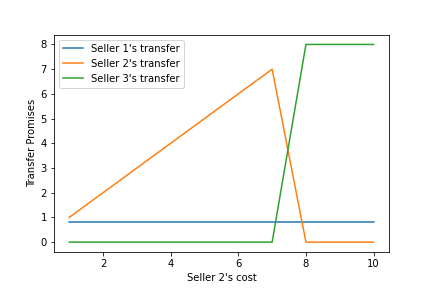
\includegraphics[width=0.8\textwidth]{\FigDir/sampleTP.png}}
	\caption{Sellers' payments under Transfer Promises}
	\label{fig:sampleTP}
\end{figure}
\hypertarget{sampleUP}{}
\begin{figure}
	\centerline{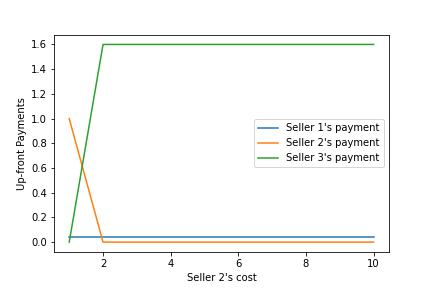
\includegraphics[width=0.8\textwidth]{\FigDir/sampleUP.png}}
	\caption{Sellers' payments under Up-front Payment}
	\label{fig:sampleUP}
\end{figure}


\subsection{Remarks}

This model gives insights on comparing different offer types. However, unlike the two previous models, this model doesn't allow for revisiting sellers who rejected previous offers.

In addition, the commitment assumption that sellers who accepts transfer promises would vote in favor of the buyer seems to be too restrictive in real-world practices. It would be interesting to study how sellers would behave if commitment is not required. A crude observation is that dispensable sellers can't be exploited as in the current model.

It would also be interesting to see how bargaining power can be implemented to this model. Both \cite{Xiao} and \cite{InOCoHoldUP}'s implementations can be incorporated.

\section{Conclusion and Potential Extensions}

\subsection{A brief comparison of the Models}

Table 1 provides a brief summary of the key features of the models described in this note.
% Comparison Table
\begin{table}
	\centering
	\caption{Model Comparison}
	\label{tab:ModComp}
	
	\begin{tabular}{lrrr}
		\toprule
		Model                    &   Xiao(2018)  & Iaryczower and Oliveros (2019) &    Chen and Zapal(2021)   \\
		\midrule
		Endogenous Sequencing    &     Yes       &               No               &            Yes            \\
		Seller Bargaining power  & Yes, via lots & Yes, via who initiates offer   &             No            \\
		Seller Heterogeneity     &     Yes       &               No               &  Yes, via different costs \\
		Allow renegotiation      &     Yes       &              Yes               &            Yes            \\	
		\bottomrule
	\end{tabular}
	
\end{table}

\subsection{Potential extensions}

In addition to all the previous remarks, one additional extension that comes to my mind is asymmetric information. All three models assume complete information, where both buyers and sellers are fully aware of which seller is being approached and whether the offer was accepted.
Completely private history may not be that interesting, since sellers have very limited information on past offers. One alternative approach may be public history among coalitions, where sellers with similar interests communicate with each other and share past offer details within the group. We can also allow information update via networks, which I'm not sure if it worth the additional complexity.


\newpage





\onlyinsubfile{% Allows two (optional) supplements to hard-wired \texname.bib bibfile:
% economics.bib is a default bibfile that supplies anything missing elsewhere
% Add-Refs.bib is an override bibfile that supplants anything in \texfile.bib or economics.bib
\IfFileExists{\econtexRoot/Add-Refs.bib}{
  % then 
  \typeout{References in Add-Refs.bib will take precedence over those elsewhere}
  \setboolean{AddRefsExists}{true}
  \setboolean{NeitherExists}{false} % Default is true
}{
  % else
  \setboolean{AddRefsExists}{false} % No added refs exist so defaults will be used
  \setboolean{BothExist}{false}     % Default is that Add-Refs and economics.bib both exist
}

% Deal with case where economics.bib is found by kpsewhich 
\IfFileExists{/usr/local/texlive/texmf-local/bibtex/bib/economics.bib}{
  % then
  \typeout{References in default global economics.bib will be used for items not found elsewhere}
  \setboolean{economicsExists}{true}
  \setboolean{NeitherExists}{false}
}{
  % else 
  \typeout{Found no global database file}
  \setboolean{economicsExists}{false}
  \setboolean{BothExist}{false}
}

\IfFileExists{economics.bib}{
  % then
  \typeout{References in economics.bib will be used for items not found elsewhere}
  \setboolean{economicsExists}{true}
  \setboolean{NeitherExists}{false}
}{
  % else 
  \typeout{Found no global database file}
  \setboolean{economicsExists}{false}
  \setboolean{BothExist}{false}
}

\ifthenelse{\boolean{BothExist}}{
  % then use both
  \typeout{bibliography{\econtexRoot/Add-Refs,\econtexRoot/\texname,economics}}
  \bibliography{\econtexRoot/Add-Refs,\econtexRoot/\texname,economics}
  % else both do not exist
}{ % maybe neither does?
  \ifthenelse{\boolean{NeitherExists}}{
    \typeout{bibliography{\texname}}
    \bibliography{\texname}}{
    % no -- at least one exists
    \ifthenelse{\boolean{AddRefsExists}}{
      \typeout{bibliography{\econtexRoot/Add-Refs,\econtexRoot/\texname}}
      \bibliography{\econtexRoot/Add-Refs,\econtexRoot/\texname}}{
      \typeout{bibliography{\econtexRoot/\texname,economics}}
      \bibliography{         \econtexRoot/\texname,economics}}
  } % end of picking the one that exists
} % end of testing whether neither exists
}
%\bibliography{economics}
\end{document}
\endinput

% If you are editing in Emacs-AucTeX, modify the lines below for your system (otherwise ignore)
% Local Variables:
% eval: (setq TeX-command-list  (assq-delete-all (car (assoc "BibTeX" TeX-command-list)) TeX-command-list))
% eval: (setq TeX-command-list  (assq-delete-all (car (assoc "BibTeX" TeX-command-list)) TeX-command-list))
% eval: (setq TeX-command-list  (assq-delete-all (car (assoc "BibTeX" TeX-command-list)) TeX-command-list))
% eval: (setq TeX-command-list  (assq-delete-all (car (assoc "Biber"  TeX-command-list)) TeX-command-list))
% eval: (add-to-list 'TeX-command-list '("BibTeX" "bibtex LaTeX/%s" TeX-run-BibTeX nil t                                                                              :help "Run BibTeX") t)
% eval: (add-to-list 'TeX-command-list '("BibTeX" "bibtex LaTeX/%s" TeX-run-BibTeX nil (plain-tex-mode latex-mode doctex-mode ams-tex-mode texinfo-mode context-mode) :help "Run BibTeX") t)
% TeX-PDF-mode: t
% TeX-file-line-error: t
% TeX-debug-warnings: t
% LaTeX-command-style: (("" "%(PDF)%(latex) %(file-line-error) %(extraopts) -output-directory=LaTeX %S%(PDFout)"))
% TeX-source-correlate-mode: t
% TeX-parse-self: t
% eval: (cond ((string-equal system-type "darwin")    (progn (setq TeX-view-program-list '(("Skim" "/Applications/Skim.app/Contents/SharedSupport/displayline -b %n LaTeX/%o %b"))))))
% eval: (cond ((string-equal system-type "gnu/linux") (progn (setq TeX-view-program-list '(("Evince" "evince --page-index=%(outpage) LaTeX/%o"))))))
% eval: (cond ((string-equal system-type "gnu/linux") (progn (setq TeX-view-program-selection '((output-pdf "Evince"))))))
% TeX-parse-all-errors: t
% End:
